\documentclass[12pt]{article}

\usepackage{graphicx}
\usepackage{float}
\usepackage[latin1]{inputenc}
%% dieses package erlaubt, bei deutscher Tastatur Umlaute, ß direkt einzugeben

\usepackage{amsmath}
\usepackage{siunitx}

\textwidth=170mm
\textheight=240mm
\hoffset= -20mm       % may need change
\voffset= -25mm       % may need change



\begin{document}

%% we do the title page ourselves
\thispagestyle{empty}     % only for frontpage
\null
\vspace{40mm}
\begin{center}
{%%%%%%%%%%%%%%%%%%%%%%%%%% Titel
\Large  The Zeemann effect
\footnote{\noindent Experiment F44, performed on 3/20/18, Tutor Pooja Surajbali, short evaluation}}\\[15mm]
%%%%%%%%%%%%%%%%%%%%%%%%%%% Authors
Lasse Gresista and Benjamin Haake

\vspace{25mm}

\parbox{0.9\textwidth}{   %% etwas schmaler als normaler Satz
Abstract:    
\small The abstract should preferentially be in English. Here we explain in a
few lines (i) what was done, and (ii) what the results were.
}
\end{center}

\vfill
%Attested as special evaluation: Date, Signature:
\vspace{20mm}


\newpage
\pagenumbering{arabic}

\section{Introduction}
In this experiment the effect of the normal Zeeman effect on the red spectral line ($\lambda\approx644nm$) of the Cadmium spectrum is observed using a Lummer-Gehrcke Plate. Additionally the wavelength of the spectral line is measured using a Czerny-Turner spectrometer. 

\subsection{The normal Zeeman Effect}
The bound electrons surrounding a nucleus can occupy different quantised energy levels. Without an external magnetic field, quantum states with the angular momentum quantum number $l$ have a degeneracy of $2l+1$. An external magnetic field $\vec{B}$ splits these energy levels. This is called the Zeeman effect. The normal Zeeman effect is the special case of all electron spins canceling each other. In a classical deviation, neglecting the spins of the electrons, the orbiting electron with an angular momentum $\vec{l}$ has a magnetic moment
\begin{equation}
\vec{\mu}_l=\frac{e}{2m_e}\vec{l}
\end{equation}
where $e$ is the electron charge and $m_e$ its mass. The interaction between the magnetic moment and the magnetic field changes the electron's potential energy. If the direction of the magnetic field is the quantisation axis $z$, and $m_l$ the magnetic quantum number, the change in potential energy can be written as
\begin{equation}
\Delta E_{pot}=-\vec{\mu}_l\cdot \vec{B}=\frac{e}{2m_e}\cdot\vec{l}\cdot\vec{B}=\mu_B \cdot m_l \cdot B
\end{equation}
where in the last step $l_z=m_l\cdot\hbar$ was used and the Bohr magneton $\mu_B=\frac{e\cdot\hbar}{2m_e}$ was introduced.

\subsection{Spectroscopy of the Zeeman Effect}
\subsubsection{Selection rules and polarisation}
If an electron transitions from an energy level $E_k$ to a lower energy level $E_i$, a photon is emitted with the energy
\begin{equation}
E_{ph}=h \cdot \nu=h \cdot \frac{c}{\lambda}=E_k-E_i
\label{eq:photonenergy}
\end{equation}
where $\nu$ is the frequency of the photon, $\lambda$ its wavelength and $c$ the speed of light. Due to momentum conversation and symmetry rules only those transitions who obey the so-called selection rules are allowed. They state that $\Delta m=0,\pm1$ and for electric dipole transitions $\Delta l=\pm1$ and $\Delta S=0$, with $S$ being the total spin of all electrons in the atom. Transitions with $\Delta m=0$ are called $\pi$-transitions and are only emitted in the transversal direction of the magnetic field. The emitted light is linearly polarised. For $\Delta m=\pm1$ the transitions are called $\sigma$-transitions. They are circularly polarised when viewed from the longitudinal direction and linearly polarised when viewed from the transversal direction.

\subsubsection{The Lummer-Gehrke plate}
To see the shift in wavelength a so-called Lummer-Gehrcke plate  will be used, which is a quartz glass plate with extremely plane parallel surfaces. Light enters the plate through a prism at an angle of nearly total internal reflection. The light then gets reflected on the surfaces inside the plate with a little bit of light escaping at each reflection with an angle of $\alpha \approx 90^\circ$ (see figure \ref{fig:lummergehrke}), which is then observed with a telescope. In a long and thin plate this way many light rays interfere with each other leading to a high resolution. For a plate in air with an index of reflection $n$, and at the limit of total internal reflection $\alpha\approx 90 ^\circ$ the optical path length difference $\Delta$ can be calculated using the following equation:
\begin{equation}
\Delta=\Delta_1-\Delta_2=2d \cdot \sqrt{n^2-1}
\end{equation}
For constructive interference $\Delta$ satisfies
\begin{equation}
\Delta=k\cdot\lambda 
\label{eq:constructive interference}
\end{equation} 
where $k$ is a whole number. Considering a change in wavelength of $\Delta\lambda$, the order $k+1$ of the wavelength $\lambda+\Delta\lambda$ and the order k of the wavelength $\lambda$ overlap for $k \cdot (\lambda+\Delta\lambda)=(k+1)\cdot\lambda$. With this condition and equation \ref{eq:constructive interference} the so-called free spectral range $\Delta\lambda$ follows from:
\begin{equation}
\Delta\lambda=\frac{\lambda^2}{2d \cdot \sqrt{n^2-1}}
\end{equation}
In an approximation to first order a small wavelength change $\delta\lambda \ll \Delta\lambda$ leads to a shift of 
\begin{equation}
\delta \lambda= \frac{\delta k}{\Delta k} \cdot \Delta\lambda
\end{equation}
where $\delta k$ is the shift in "order" resulting from the wavelength shift corresponding to a certain shift in the position of the line on the detector and $\Delta k$ is the difference between to nearby orders, which means $\Delta k=1$. With the above equations the final result is:
\begin{equation}
\delta\lambda=\delta k \cdot \frac{\lambda^2}{2d\cdot\sqrt{n^2-1}}
\label{dlambda}
\end{equation}
\begin{figure}
\centering
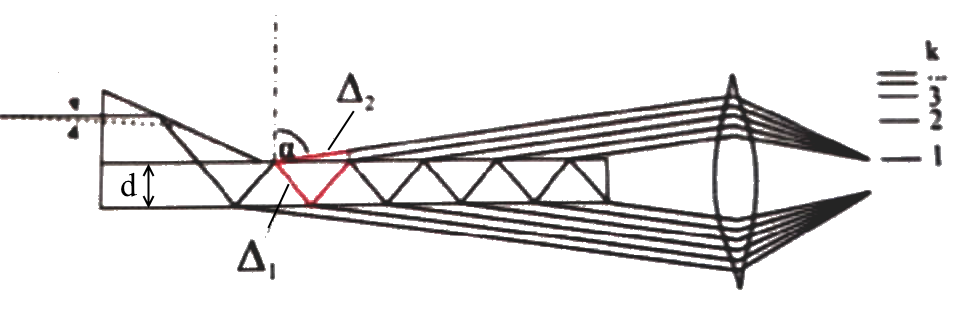
\includegraphics[width=0.5\textwidth]{fig/lummergehrke.png}
\caption{Schematic of the Lummer-Gehrke plate}
\label{fig:lummergehrke}
\end{figure}


\section{Setup of the experiment}
In both parts of the experiment the red line of a cadmium lamp will be observed, which arises from the transition between the two excited levels $^1D_2\rightarrow \ ^1P_1$ in the fifth shell of Cd.
\subsection{Part 1: Spectroscopy of the Zeeman Effect}
To investigate the normal Zeeman effect the light of a Cadmium lamp is observed through a Lummer-Gehrcke plate. The pole pieces of an electromagnet are positioned on opposing sides of the Cd lamp. The set-up is turnable and the pole pieces have a hole in the middle, which makes it possible to observe both transversal and longitudinal directions. The spectra are taken through a red light filter with a telescope and a CCD-Camera. The magnetic field strength is measured with a Gaussmeter.
\subsection{Part 2: Precision Spectroscopy}
To determine the absolute wavelength of the red Cd line a Czerny-Turner Spectrometer is used. Light entering the spectrometer through an entrance split is focused by a concave mirror on a grating, where it gets diffracted. The diffracted light then is focused by another concave mirror onto a CCD camera. The light of the Cd lamp and the neon lamp, which is used for the calibration of the setup, is connected to the spectrometer using an optical fiber and two lenses to focus the light on the entrance slit. 

\section{Execution}
\subsection{Part 1: Spectroscopy of the Zeeman Effect}
To convert the current applied to the electromagnets into the magnetic field strength, the field strength was measured for currents from $1-14A$ in steps of $1A$. This was done for ascending and descending currents to account for the hysteresis effect. Each measurement of a magnetic field strength measurement was done 3 times and an average was taken.
\\Next the light of the Cd lamp with the magnetic field turned on was observed in both longitudinal and transversal directions. In the transversal direction spectra were recorded for a current of $I=10A$, $I=12$ and $I=14A$ in ascending order. Additionally $\lambda/4$ and polarisation filters were used to determine the polarisation of the emitted light. 
\subsection{Part 2: Precision Spectroscopy}
Spectra were taken with a grating of $1800\, \text{lines}/mm$ and an integration time of $60 s$. First the region of the neon spectrum with wavelengths of around $630nm-655nm$ was observed. Without changing the setup except now using the Cd lamp the same region of the Cd spectrum was observed. 
\section{Evaluation}
	To obtain the magnetic field strength from the applied current in later parts of the experiment a linear fit to the last few ascending measurements was made. 
\subsection{Part 1: Spectroscopy of the Zeeman Effect}
	Since the transversal lines vanish for certain configurations of the polarisation filter and the $\frac{\lambda}{4}$-plate has no effect, we conclude that they are linearly polarised. Additionally, the polarisations of the $\sigma$- and $\pi$-line are perpendicular to each other, since the lines vanish for orientations of the polarisation filter related by a rotation of $\ang{90}$.\\
	Similarly, the $\sigma$-lines must be circularly polarised in longitudinal direction since they vanish for certain configurations where both filters were applied simultaneously ($\frac{\lambda}{4}$-plate first). Since they vanish at angles related by a rotation of $\ang{90}$ of the polarisation filter, the orientation of the polarisation must be different, i.e. counter-clockwise in one case and clockwise in the other.\\
\begin{figure}
\centering
\label{fig:master12_A}
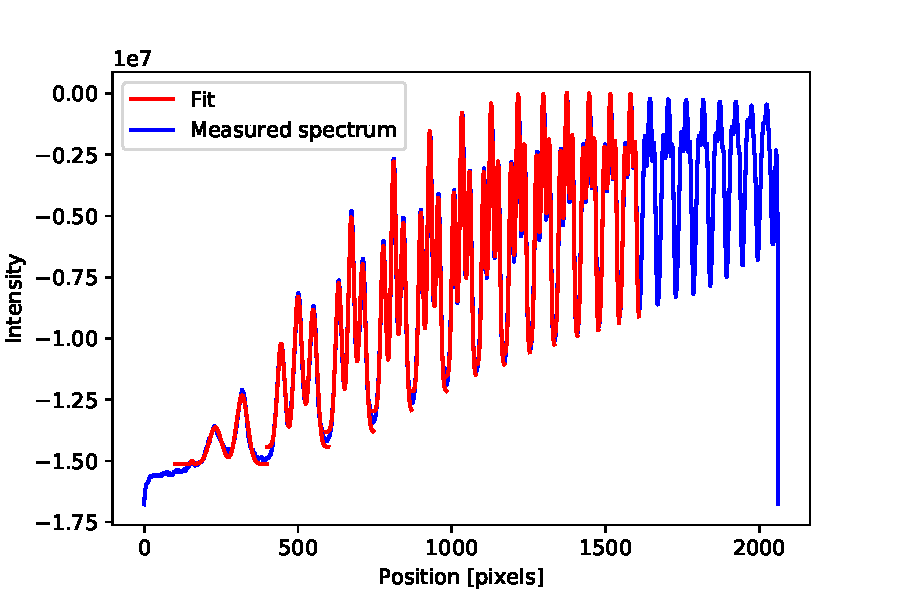
\includegraphics[width=0.9\textwidth]{fig/master12A.pdf}
\caption{Observed transversal diffraction pattern at $12A$}
\end{figure}
	After the positions of all peaks (in transversal direction) had been determined by fitting gaussians (exemplified by figure \ref{fig:master12_A} for the $12A$ measurement), the order of interference was plotted and fitted against the positions of the $\pi$-lines. From the resulting parabolic function the positions of the $\sigma$-lines were assigned an interference order $k+\delta k$ where $k$ is the order of the associated $\pi$-line. The shift in wavelength can the be calculated via equation \ref{dlambda}. The energy difference is then given by:
	\begin{align}
		\Delta E&=hc\;\Bigl(\frac{1}{\lambda}-\frac{1}{\lambda+\delta \lambda} \Bigr) 
		\label{dE1}\\
		&=\mu_BBm_l
		\label{dE2}
	\end{align}
	The Bohr magneton $\mu_B$ can now be determined by using equation \ref{dE1} to calculate $\Delta E$ and equation \ref{dE2} to obtain:
	\begin{equation}	
		\mu_B=\biggl| \frac{\Delta E}{B}\biggr|
	\end{equation}
	The results are displayed in table \ref{resultsP1}, the values for the magnetic field were calculated from the linear fit.
	\begin{table}[H]
		\centering
		\begin{tabular}{cccccc}
			I[\si{\ampere}]&B[\si{\milli\tesla}]&$\delta\lambda_l$[\si{\pico\metre}]&$\mu_{B,l}$[\si{10^{-24}\joule\per\tesla}]&$\delta\lambda_r$[\si{\pico\metre}]&$\mu_{B,r}$[\si{10^{-24}\joule\per\tesla}]\\
			$10,0\pm 0,2$&$525\pm 19$&$-11,23\pm 0,46$&$10,25\pm 0,43$&$10,00\pm 0,44$&$9,13\pm 0,42$\\
			$12,0\pm 0,2$&$589\pm 19$&$-13,06\pm 0,48$&$10,63\pm 0,40$&$11,91\pm 0,47$&$9,69\pm 0,39$\\
			$14,0\pm 0,2$&$652\pm 19$&$-14,12\pm 0,48$&$10,38\pm 0,37$&$12,80\pm 0,47$&$9,40\pm 0,35$\\
			\label{resultsP1}
		\end{tabular}
		\caption{Determining the Bohr magneton}
	\end{table}
One measurement deviates significantly from the literature value of $\mu_B=9,274\, 10^{-24}\si{\joule\per\tesla}$ and the values on the left side are higher, suggesting a systematic error that was not accounted for.

\subsection{Part 2: Precision Spectroscopy}
	The positions of the peaks were determined as before and wavelengths were assigned to the Neon-lines. From these, a linear fit was produced that was used to determine the wavelengths of the lines in the Cadmium spectrum. The spectrum of the Cadmium lamp can be seen in figure \ref{fig:cd_spectrum}.
\\
\begin{figure}
\centering
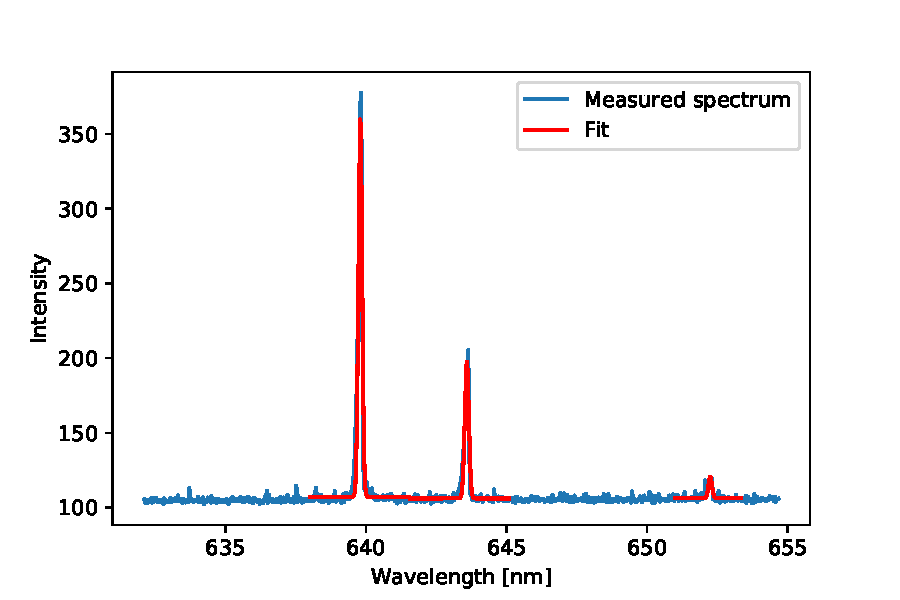
\includegraphics[width=0.9\textwidth]{fig/cd_spectrum_nm.pdf}
\caption{Spectrum of the Cd-lamp}
\label{fig:cd_spectrum}
\end{figure} 
	The element that fitted best was Mercury (Hg), but there is no known reason for the lamp to contain it. Another explanation might be Thorium, which might be used for the electrodes (for exact values, see Discussion).

\section{Discussion}

When observing the Cadmium lamp trough the Lummer-Gherke plate one could qualitatively see very well how the magnetic field affects the light emitted by the Cadmium lamp. In the transversal direction $\pi$- and $\sigma$-lines are emitted both being linearly polarised, and in the longitudinal direction two $\sigma$-lines are emitted which are circularly polarised with opposing directions of rotation. There was also a faint $\pi$-line visible in the longitudinal direction, probably due to reflections.
\\When determining the wavelength shift $\delta \lambda$ for both $\sigma$-lines in the transversal direction, the left line consistently produced slightly higher values for $\mu_B$. One source of error could be the growing background noise in the spectrum. This was not accounted for in the fit, even though you see a noticeable rise comparing the left and right $\sigma$-peak of the same order. 
\\To obtain a spectrum (intensity against position in pixels) out of an image taken with the CCD camera, a hand drawn reference line was used to determine the alignment of the spectral lines. This might have also shifted the spectrum to one side, but since the results for all three magnetic field strengths showed a deviation in the same direction, it's unlikely that this is the cause for the higher values. 
\\When comparing the experimental values for the Bohr magneton $\mu_B$ to the literature value ($\mu_B=9.247\cdot10^{-24}J/T$) there is only one significant deviation, and the best value was obtained with the right $\sigma$-peak and a current of I=12A, where the deviation is less than 1$\sigma$ ($\mu_B=(9.40\pm0.35)\cdot10^{-24}J/T$. All experimental values are higher than the literature value, especially the ones for the left side. This suggests another unaccounted systematic error.
\\In the second part of the experiment the wavelength of the observed Cd-line was determined to be $\lambda_{Cd}=(643.59\pm0.19)nm$. The literature value is $\lambda_{Cd, lit}=643.847nm$ \cite{nist}, so the deviation is less than 2$\sigma$. 
\\The other two wavelengths in the spectrum were determined to be $\lambda_1=(639.80\pm0.17)nm$ and $\lambda_2=(652.25\pm0.26)nm$. It was tried to identify the element emitting those lines using the NIST Atomic Spectra Database. The element with the best fitting spectral lines was Mercury, since it has two lines at $\lambda_{Hg,1}=(639.4890\pm0.0003)nm$ and $\lambda_{Hg,2}=(652.1092\pm0.0003)nm$. This means there is only a 1$\sigma$ and 2$\sigma$ deviation. All other elements either had a significant deviations or had other spectral lines with high intensity that would have also appeared in our image if the element was present. It is however no reason known why mercury should be in a cadmium lamp. Another suggestion is Thorium, which is sometimes used as the material for the cathode of cadmium lamps. It has two spectral lines at $\lambda_{Th,1}=(640.644609\pm0.000006)nm$ and $\lambda_{Th,2}=(652.204346\pm0.00013)nm$. The second wavelength fits well with a deviation below 1$\sigma$, the first line deviates significantly. There are however many more spectral lines in the same wavelength range with high relative intensity that are not appearing in our spectrum. To definitively identify the element, more information on the cadmium lamp or the set-up in general seems to be necessary. 



\newpage
\begin{thebibliography}{00}   % {00}: max 2-stellige Referenznummer

\bibitem{sc} Zeemann-effect (2010)
\bibitem{nist} Kramida, A., Ralchenko, Yu., Reader, J., and NIST ASD Team (2018). NIST Atomic Spectra Database (ver. 5.5.6), [Online]. Available: https://physics.nist.gov/asd [2018, April 16]. National Institute of Standards and Technology, Gaithersburg, MD. 

\end{thebibliography}
\end{document}
